\section{Problem 2}
\label{part2}
\subsection*{Question}
\begingroup
\begin{verbatim}
Create an ASCII and JPEG dendrogram that clusters (i.e., HAC)
the most similar blogs (see slides 12 & 13).  Include the JPEG in
your report and upload the ascii file to github (it will be too
unwieldy for inclusion in the report).
\end{verbatim}
\subsection{Answer}
\begin{enumerate}
\item The script show in Listing \ref{lst:dendro-code} uses the \emph{Toby Segaran's clusters.py} code in Listing \ref{lst:clusters} and produces the Dendrogram shown in Figure \ref{Dendrogram}

\item The printclust function on line 8 in Listing \ref{lst:dendro-code} prints the dendrogram. The drawdendrogram function on line 11 saves a JPEG of the dendrogram.

\item The ascii file of the dendrogram is uploaded to github, and the file name is \emph{ascii-dendrogram.txt}.

\item Unfortunately, it is difficult to see, but this dendogram shows that the blogs calculated to be most like \emph{F-Measure} are split into two clusters, the blogs in the first cluster are \emph{YOUNGEST INDIE} and \emph{Music Liberation}, the blogs in second cluster are \emph{The Devils Music} and \emph{McCrak's Juke}. 
\item The blog calculated to be most like \emph{Web Science and Digital Libraries Research Group} are \emph{Koranteng's Toli} and \emph{words of advance for young people}.
\end{enumerate}



\lstinputlisting[language=python, frame=single,breaklines=true, caption={Python code for grabbing number of pages for each blog},captionpos=b, numbers=left, showspaces=false,label=lst:dendro-code, showstringspaces=false, basicstyle=\footnotesize]{questions/q2/q2dendo.py}
\newpage
\clearpage

\begin{figure}[ht]    
    \begin{center}
        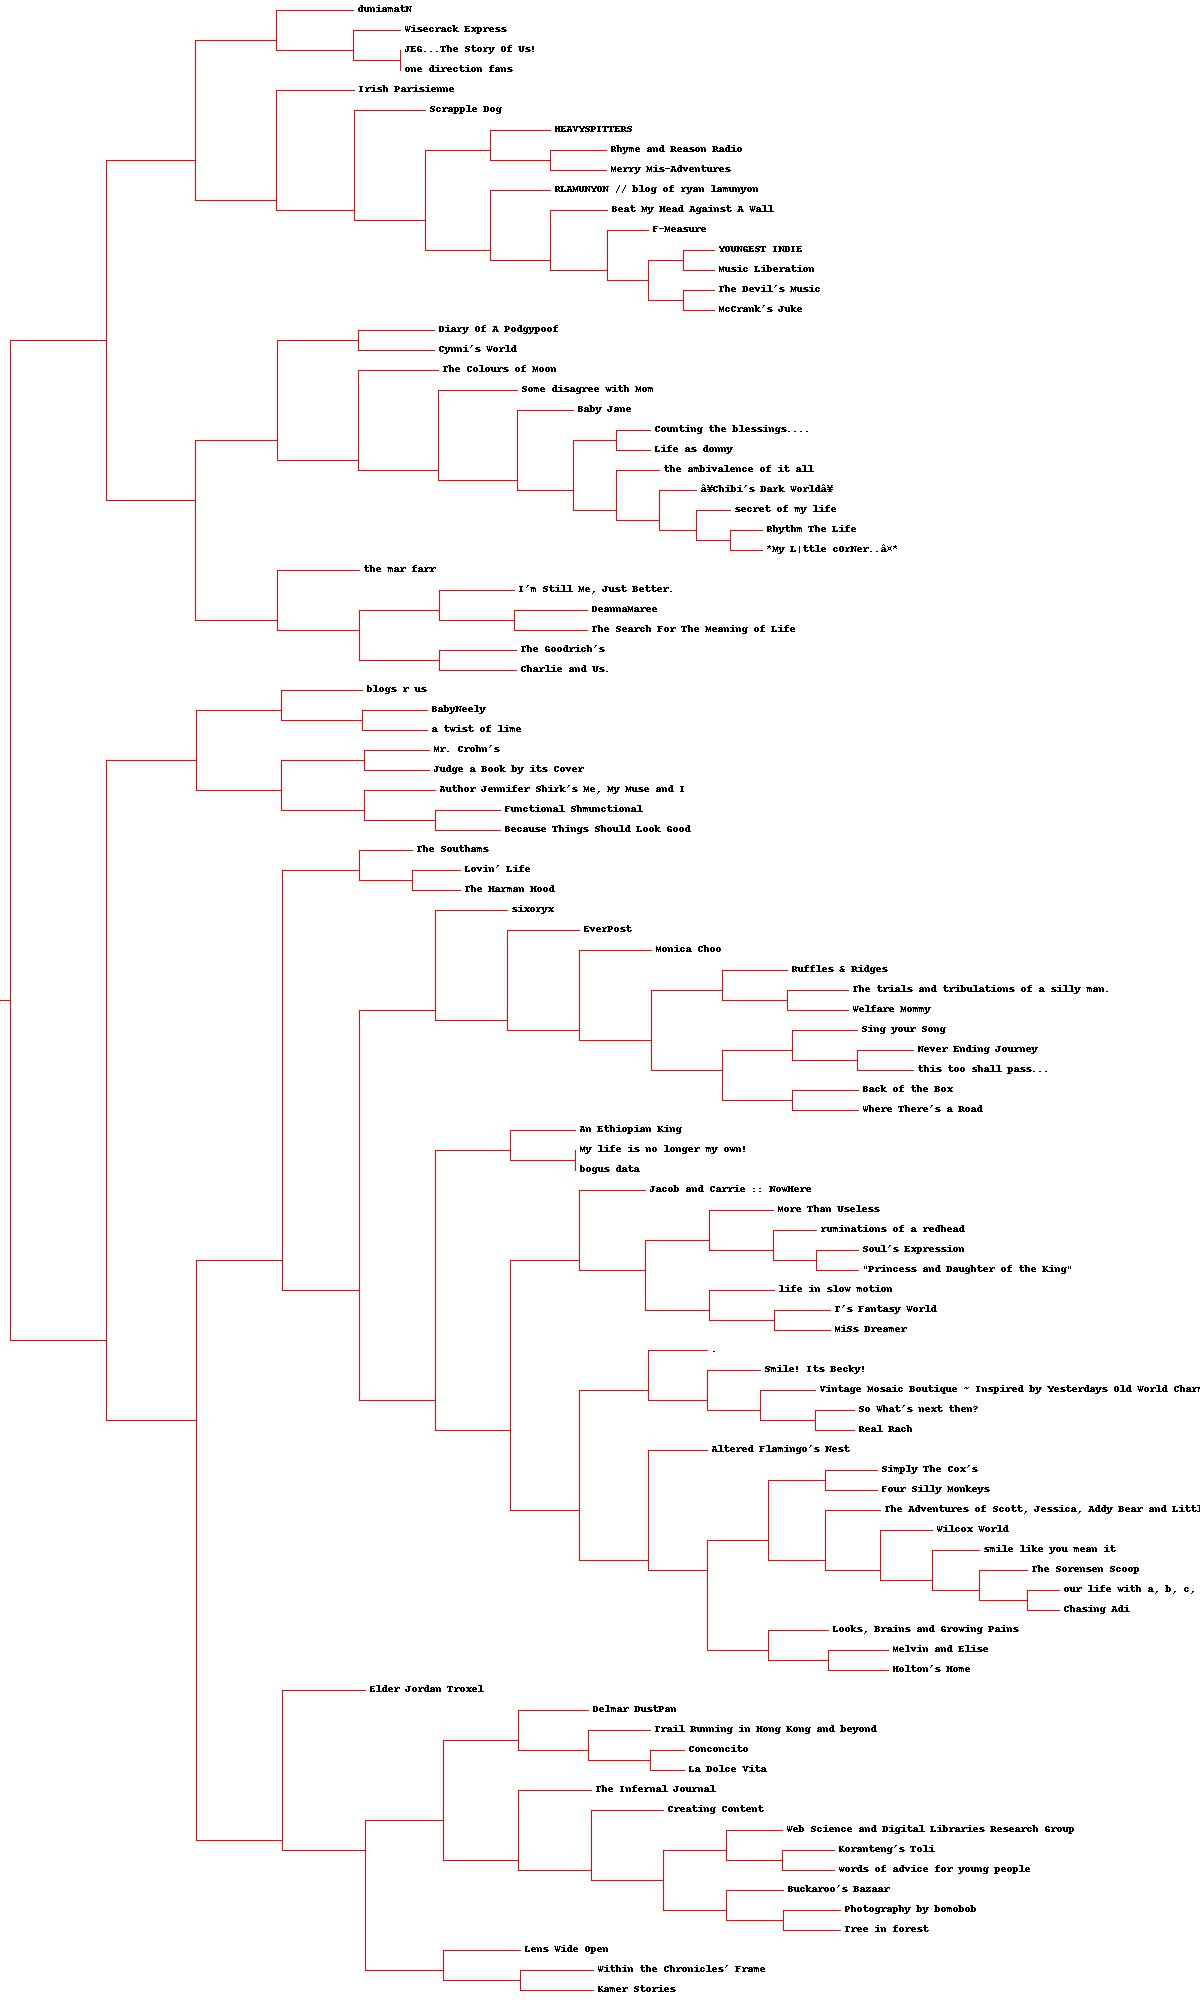
\includegraphics[scale=0.26]{questions/q2/blogclust.jpg}
        \caption{Dendrogram Produced by Program in Listing \ref{lst:dendro-code}}
        \label{Dendrogram}
    \end{center}
\end{figure}

\newpage
